	\clearpage
\section{Ablauf}\label{sec:Ablauf}
Ein Mesh Benchmark folgt einem klar definierten Ablauf. Die Abbildung \ref{fig:MeshTestkablauf} beschreibt den konzeptionellen Ablauf unabhängig vom zu testenden Mesh Protokoll.

\begin{figure}[H]
	\centering
	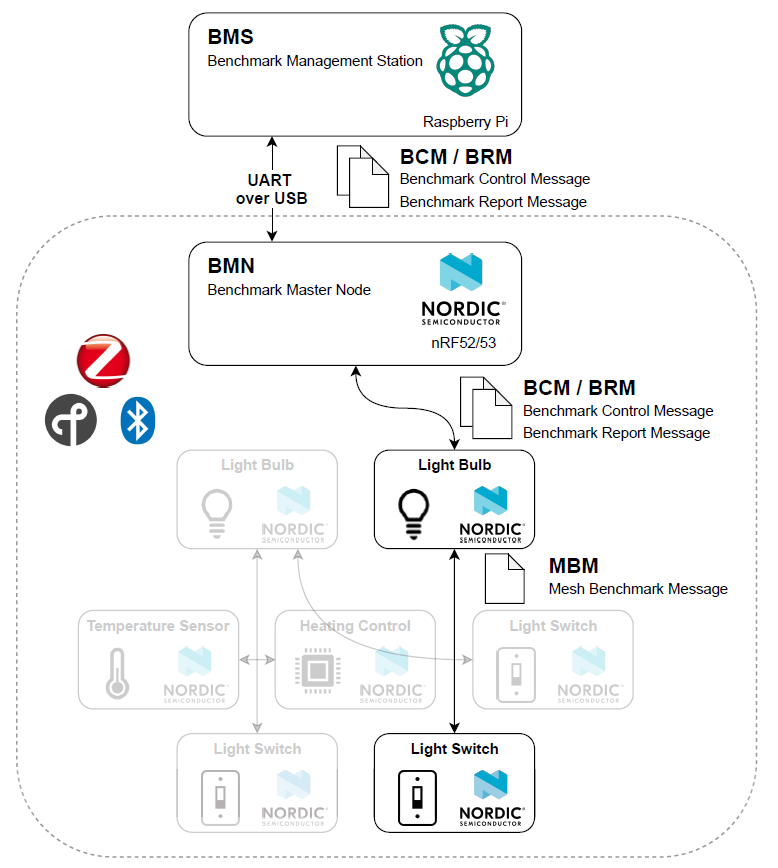
\includegraphics[width=1.0\textwidth]{Mesh_Testablauf.png}
	\caption{Konzeptschema für den Ablauf eines Mesh Benchmarks.}\label{fig:MeshTestkablauf}
\end{figure}

\begin{enumerate}
	\item \textbf{Benchmark User-Init:}\\
	Auf dem Webinterface des BMS werden die gewünschten Parameter definiert und der Benchmark durch den Benutzer gestartet.
	\item \textbf{Benchmark Init BMN:}\\
	Die Parameter werden an den BMN übergeben welcher diese wiederum an alle teilnehmenden BSN weiterleitet. Mit einem Startsignal vom BMN wird der Benchmark auf den BSN gestartet.
	\item \textbf{Benchmark Prozess:}\\
	Die BSN führen den Benchmark Prozess mit den definierten Parametern aus. Dies geschieht autonom und jeweils nur zwischen den entsprechenden BSN die in einer direkten Beziehung zueinander stehen (siehe Mesh Beziehungen \ref{subsec:MeshBeziehungen}). Die entstehenden Messdaten werden auf den BSN zwischen gespeichert.
	\item \textbf{Reporting:}\\
	Nach Ablauf der Benchmark Zeit werden die Messdaten an den BMN übertragen. Dies erfolgt gesteuert durch den BMN welcher die Daten bei einem BSN nach dem anderen abfragt und direkt an das BMS weiterleitet.
	\item \textbf{Finish:}\\
	Der BMN kontrolliert ob er die Daten von sämtlichen BSN korrekt auslesen konnte und bestätigt das Ende der Messung gegenüber dem BMS.
	\item \textbf{Auswertung:}\\
	Das BMS beendet den Benchmark Vorgang, speichert die Messdaten in seiner Datenbank ab und bereitet diese grafisch auf. 
\end{enumerate}








